\section{Ecuación de estado cúbica}
 La presión es el cálculo mas sencillo que podemos realizar con la ecuación de estado cúbica.

\begin{equation}
	p = \frac{R T}{v-b} - \frac{a}{v^2 +u b v + w b^2 }
\end{equation}

 Crearemos una clase en java que use la librería Materia y realize una gráfica de presión contra volumen a una temperatura determinada.

%\pgfplotstabletypeset{plotdata/pressurevolume.dat}%no es necesario mostrar la tabla

\begin{tikzpicture}
\begin{axis}
\addplot[blue]table{plotdata/pressurevolume.dat};
\end{axis}
\end{tikzpicture}


\begin{tikzpicture}
\begin{axis}
\addplot3[surf,
colormap={blueblack}{color=(white) color=(blue)},
domain=0:1]table{plotdata/pressurevolumetemperature.dat};
\end{axis}
\end{tikzpicture}


\begin{lstlisting}[label=se,caption=Some Code]
Cubic cubic = new Cubic();
//parametros de van der waals para el heptano
double a = 3107000.0;
double b = 0.2049;


double min_volume = 0.245;
double max_volume = 2.06;

int n = 100;
double pass = (max_volume- min_volume)/n;

PrintWriter writer = new PrintWriter(fileName, "UTF-8");
writer.println(" Volumen Presion");
for(int i=0;i < n; i++){
	double volume = min_volume + pass*i;
	double pressure = cubic.calculatePressure(300, volume, a, b);
	
	writer.println(" "+ volume + " " + pressure);
}
writer.close();		
\end{lstlisting}


\begin{equation}
	b_i = \Omega_b \frac{R T_{ci}}{p_{ci}} \qquad a_i = \Omega_a \frac{\left(R T_{ci}\right)^2}{p_{ci}} \alpha_i
\end{equation}

\begin{figure}[!h]
  
  \centering
    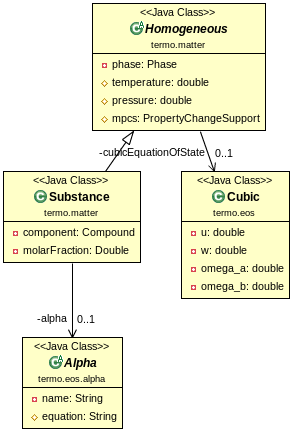
\includegraphics[scale=0.7]{cubic.png}
    \caption{A picture of a gull.}
\end{figure}








